\section{A spatial representation of interval models}\label{sec:compass}

Let us now introduce some basic definitions and notation which will be
extensively used in the following, concluding the section with the notion of compass structure. Given a $\D$ formula $\varphi$,
we define the \emph{closure of $\varphi$}, denoted by
$\CL(\varphi)$, as the set of all subformulas $\psi$ of $\varphi$ and of their
negations $\neg\psi$ (we identify $\neg\neg \psi$ with $\psi$). %Moreover we define the notion of $\varphi$-atom as follows.

\begin{definition}\label{def:d-atom}
Given a $\D$-formula $\varphi$, a $\varphi$-atom $A$ is a subset of
$\CL(\varphi)$ such that: 
\begin{itemize}
    \item  for every $\psi \in \CL(\varphi)$, $\psi \in A$ if and only if $\neg\psi \notin A$, and
    \item for every $\psi_1 \vee \psi_2 \in \CL(\varphi)$, $\psi_1 \vee \psi_2 \in A$ if and only if $\psi_1 \in A$ or $\psi_2 \in A$.
\end{itemize}
\end{definition}

The idea underlying atoms is to enforce a \lq\lq local\rq\rq{} (or Boolean) form of consistency among the formulas it contains, that is, a $\varphi$-atom $A$ is a \emph{maximal, locally consistent subset} of $\CL(\varphi)$. As an example, $\neg(\psi_1 \vee \psi_2) \in A$ if and only if $\neg\psi_1\in A$ and $\neg\psi_2\in A$. However, note that the definition does not set any constraint on $\hsD\psi$ formulas, hence the word ``local''.
We denote the set of all $\varphi$-atoms as $\cA_\varphi$; its cardinality is clearly bounded by $2^{|\varphi|}$ (by the first point of Definition~\ref{def:d-atom}). Atoms are connected by the following binary relation $\Dphi$.

\begin{definition}\label{def:Dphi-relation}
Let $\Dphi$ be a binary relation over $\cA_\varphi$ such that, for each pair of atoms $A, A' \in \cA_\varphi$, $A \Dphi A'$ holds if and only if both $\psi \in A'$ and $\hsDu\psi \in A'$ for each formula $\hsDu\psi \in A$.
\end{definition}

Let $A$ be a $\varphi$-atom. We denote by $\reqD(A)$ the set $\{\psi \in \CL(\varphi) \mid \hsD \psi \in A\}$ of \lq\lq \emph{temporal requests}\rq\rq{} of $A$. In particular, if $ \psi \notin \reqD(A)$, then $\hsDu \neg \psi \in A$ (by the definition of $\varphi$-atom). Moreover, we denote by $\REQ_{\varphi}$ the set of all  arguments of $\D$ formulas in $\CL(\varphi)$, namely, $\REQ_{\varphi}=\{ \psi \mid \hsD \psi\in \CL(\varphi)\}$. Finally, we denote by $\obsD(A)$ the set $\{\psi \in A \mid \psi \in \REQ_{\varphi}\}$ of \lq\lq \emph{observables}\rq\rq{} of $A$. 

It is easy to prove by induction the next proposition stating that, once the proposition letters of $A$ and its temporal requests are fixed, $A$ is determined.
\begin{proposition}\label{prop:unique}
    For any $\D$ formula $\varphi$,
    given a set $R \subseteq \REQ_{\varphi}$ and a set $P \subseteq \CL(\varphi)\cap \AP$, there exists a unique $\varphi$-atom $A$ that satisfies $\reqD(A)=R$ and $A\cap \AP = P$.
\end{proposition} 

We now provide a natural interpretation of $\D$\ over grid-like
structures, called \emph{compass structures}, by exploiting the existence
of a natural bijection between intervals $[x,y]$ and 
points $(x,y)$, with $x \leq y$, of an $\mathpzc{S}\times \mathpzc{S}$ grid, where $\mathbb{S} = (\mathpzc{S},<)$ is a finite linear order. Such an interpretation was originally proposed by Venema in~\cite{venema1990},
and it can also be given for $\HS$ and all its (other) fragments.


\begin{figure}[tb]
%\vspace*{-0.6cm}
\centering
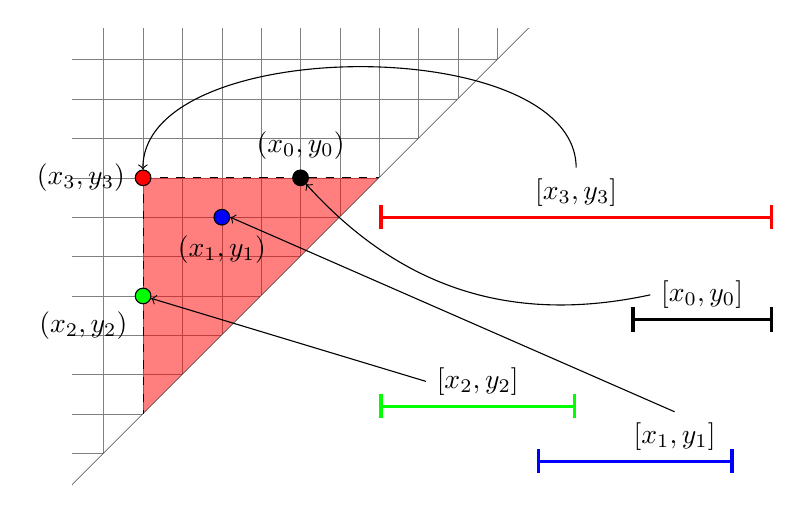
\begin{tikzpicture}[scale=1]

\draw[step=0.5cm,gray,very thin] (-2.9,-2.9) grid (2.9,2.9);
\fill[color=red, opacity=.5] (-2,1) -- (1,1)-- (-2,-2);
\draw (-2.9,-2.9) -- (2.9,2.9);
\fill[color=white] (-2.9,-2.9) -- (2.9,2.9) -- (2.9,-2.9);
\draw[dashed] (-2,1) -- (-2, -2);
\draw[dashed] (-2,1) -- (1, 1);

\node[shape=circle,draw=black,inner sep=2pt,fill=black, label={above :$(x_0,y_0)$}](A) at (0,1) {};

\node[shape=circle,draw=black,inner sep=2pt,fill=red, label={left :$(x_3,y_3)$}](C) at (-2,1) {};

\node[shape=circle,draw=black,inner sep=2pt,fill=blue, label={below :$(x_1,y_1)$}](B) at (-1,0.5) {};
\node[shape=circle,draw=black,inner sep=2pt,fill=green, label={below left:$(x_2,y_2)$}](D) at (-2,-0.5) {};

\pgftransformshift{\pgfpoint{4cm}{-0.5cm}}

\draw[very thick,|-|] (0.2,-0.3) -- (2,-0.3)node[pos=0.5, above](AI) {$[x_0,y_0]$};

\draw(AI.west) edge[->, bend left] (A);

\draw[very thick,|-|,red] (-3,1) -- (2,1)node[pos=0.5, above=0.001cm,black](CI) {$[x_3,y_3]$};

\draw(CI.north) edge[->, bend right=90, looseness=0.8] (C);


\draw[very thick,|-|,blue] (-1,-2.1) -- (1.5,-2.1)node[pos=0.7, above=0.001cm,black](BI) {$[x_1,y_1]$};

\draw(BI.north) edge[->] (B.east);

\draw[very thick,|-|,green] (-3,-1.4) -- (-0.5,-1.4)node[pos=0.5, above=0.001cm,black](DI) {$[x_2,y_2]$};

\draw(DI.west) edge[->] (D);

\end{tikzpicture}
%\vspace*{0.5cm}
\caption{Correspondence between intervals and points of the compass structure.}\label{fig:compassstructure}
%
\end{figure}

As an example, Figure~\ref{fig:compassstructure} shows four intervals
$[x_0,y_0],\ldots,[x_3,y_3]$, respectively represented by the points in the grid $(x_0,y_0),\ldots,(x_3,y_3)$, such that: 
\begin{itemize}
    \item $[x_0,y_0], [x_1,y_1], [x_2,y_2]\subint [x_3,y_3]$, 
    \item $[x_1,y_1] \ssubint [x_3,y_3]$, and 
    \item $[x_0,y_0], [x_2,y_2]\not\!\!\ssubint [x_3,y_3]$. 
\end{itemize}
The red 
region highlighted in Figure~\ref{fig:compassstructure} contains all and only the points $(x,y)$ such that $[x,y]\subint[x_3,y_3]$.
Allen interval relation \emph{contains} can thus be represented as a spatial relation between pairs of points. In the following, we make use of $\subint$ also for relating points, i.e., given two points $(x,y),(x',y')$ of the grid,
$(x',y')\subint (x,y)$ if and only if $(x',y')\neq (x,y)$ and  $x\leq x'\leq y'\leq y$.
%
Compass structures, repeatedly exploited in the following to establish the next complexity results, % as an alternative (and possibly easier to understand) interpretation to linear orders. 
can be formally defined as follows.

\begin{definition}\label{def:compassstructure}
Given a finite linear order $\mathbb{S} = (\mathpzc{S}, <)$ and a $\D$ formula $\varphi$, a  \emph{compass}
$\varphi$-\emph{structure} is a pair $\cG=(\bbP_\bbD,\cL)$,
where $\bbP_\bbD$ is the set of points of the form $(x,y)$,
with $x,y \in \mathpzc{S}$ and $ x\leq y$, and $\cL$ is a function that
maps any point $(x,y)\in\bbP_\bbD$ to a $\varphi$-atom $\cL(x,y)$
in such a way that for every pair of points $(x,y)\neq(x',y')\in\bbP_\bbD$ ,
        if $x\leq x'\leq y'\leq y$ then $\cL(x,y) \Dphi \cL(x',y')$
        (\emph{temporal consistency}).
\end{definition}
%
Due to temporal consistency, the following important property holds in compass structures.
%
\begin{lemma}\label{lem:transitive_req}
Given a compass $\varphi$-structure $\cG=(\bbP_\bbD,\cL)$,
for all pairs of points $(x',y'), (x,y)\in \bbP_\bbD$,
if $(x',y')\subint (x,y)$,
then $\reqD(\cL(x',y')) \subseteq \reqD(\cL(x,y))$ and $\obsD(\cL(x',y')) \subseteq \reqD(\cL(x,y))$.
\end{lemma}
%
\begin{proof} 
%Let us consider a pair of points $(x',y'), (x,y)\in \bbP_\bbD$ such that $(x',y')\subint (x,y)$.
By Definition \ref{def:compassstructure} we have  $\cL(x,y) \Dphi \cL(x',y')$.
Let us assume by contradiction that there exists  $\psi \in \reqD(\cL(x',y'))\setminus \reqD(\cL(x,y))$. By definition of $\reqD$ and by Definition  \ref{def:d-atom}, we have that 
$\psi \in \reqD(\cL(x',y'))$ 
implies   $\hsD\psi \in \cL(x',y')$, and
$\psi \notin \reqD(\cL(x,y))$ 
implies   $\neg\hsD\psi =\hsDu \neg \psi \in \cL(x,y)$. Since $\cL(x,y) \Dphi \cL(x',y')$,
then $\hsDu \neg \psi \in \cL(x',y')$ and thus we can conclude that
both $\hsDu \neg \psi$ and $\hsD \psi$ belong to $\cL(x',y')$ (contradiction).

$\obsD(\cL(x',y')) \subseteq \reqD(\cL(x,y))$ can analogously be proved by contradiction.
\end{proof}

\emph{Fulfilling} compass structures are defined as follows.
%
\begin{definition}\label{def:fulfillingcompass}
%Given a finite linear order $\mathbb{S} = \langle S, <\rangle$, a $\D$-formula $\varphi$ and 
A compass $\varphi$-structure
$\cG=(\bbP_\bbD,\cL)$ is said to be \emph{fulfilling}
if, for every point $(x,y)\in\bbP_\bbD$ and each formula 
$\psi\in \reqD(\cL(x,y))$, 
there exists a point $(x',y')\subint (x,y)$ in $\bbP_\bbD$ such that 
$\psi \in \cL(x',y')$.
\end{definition}
Note that if $\cG$ is fulfilling, then $\reqD(\cL(x,x))=\emptyset$ for all points ``on the diagonal'' $(x,x)\in\bbP_\bbD$.
%
%The following proposition states that satisfiability of a
%$\D$ -formula $\varphi$ is reducible to the problem of deciding whether there exists a fulfilling compass $\varphi$-structure featuring
%$\varphi$.
%
We say that a compass $\varphi$-structure $\cG=(\bbP_\bbD,\cL)$
\emph{features} a formula $\psi$ if there exists a point $(x,y)\in\bbP_\bbD$
such that $\psi \in \cL(x,y)$.
The following result holds.
%
\begin{proposition}\label{prop:compassstructure}
A $\D$ formula $\varphi$ is satisfiable if and only if there exists a fulfilling compass $\varphi$-structure that
features it.
\end{proposition}

In a fulfilling compass $\varphi$-structure  $\cG=(\bbP_\bbD,\cL)$, where $\mathpzc{S}=\{0,\ldots,t\}$, w.l.o.g., we will sometimes assume  $\varphi$ to be satisfied by the maximal interval $[0,t]$, that is, $\varphi\in\cL(0,t)$.%~\cite{sala2010decidability}.

The notion of homogeneous models directly transfers to compass structures.
%
\begin{definition}\label{def:hom_compass}
A compass $\varphi$-structure $\cG=(\bbP_\bbD,\cL)$ is \emph{homogeneous}
if, for every point $(x,y)\in \bbP_\bbD$ and each proposition letter $p\in \AP$,
we have that $p\in \cL(x,y)$ if and only if $p\in \cL(x',x')$ for all $x\leq x'\leq y$.
\end{definition}

Proposition \ref{prop:compassstructure} can be tailored to homogeneous compass structures.
%
\begin{proposition}\label{prop:satiffcompass}
A $\hsDhom$ formula $\varphi$ is satisfiable if and only if there exists a fulfilling homogeneous compass $\varphi$-structure that
features it.
\end{proposition}